%!TEX root = 0_document_de.tex
\section{Appendix}
\subsection{Passive Front Cover Heating}
To defrost ice accumulated on the outer surface of the LiDAR sensor without an active heating element, warm air need to be blown over the inner surface of the front cover, in the same way as an automobile windshield is defrosted. The air within a closed sensor is only weakly circulating though, with a wind speed of less than 1 km/h. Consider a front cover with a thickness of $d = 4 \unit{mm}$ and thermal conductivity of \(k = 1 \,\, \unit{W/m\cdot K}\). The outside ambient temperature is \(T_{amb} = -5\dC\) and the convection heat transfer coefficient is \(h_{out} = 25 \, \, \unit{W/m²\textbullet K}$, which corresponds to a front cover exposed to a wind speed of about 1 km/h. Also consider a sensor with a front cover area of 45 \unit{cm^2} and an average power consumption of 5 \unit{W}. As shown in the following, the outer front cover surface is not heated up to the melting point. Even when increasing the power consumption and using a thinner front cover, the passive heating is not sufficient to cause the accumulated ice to begin melting if the surface is exposed to slightly higher wind speeds or lower ambient temperatures.


\begin{figure} [H]
	\centering
	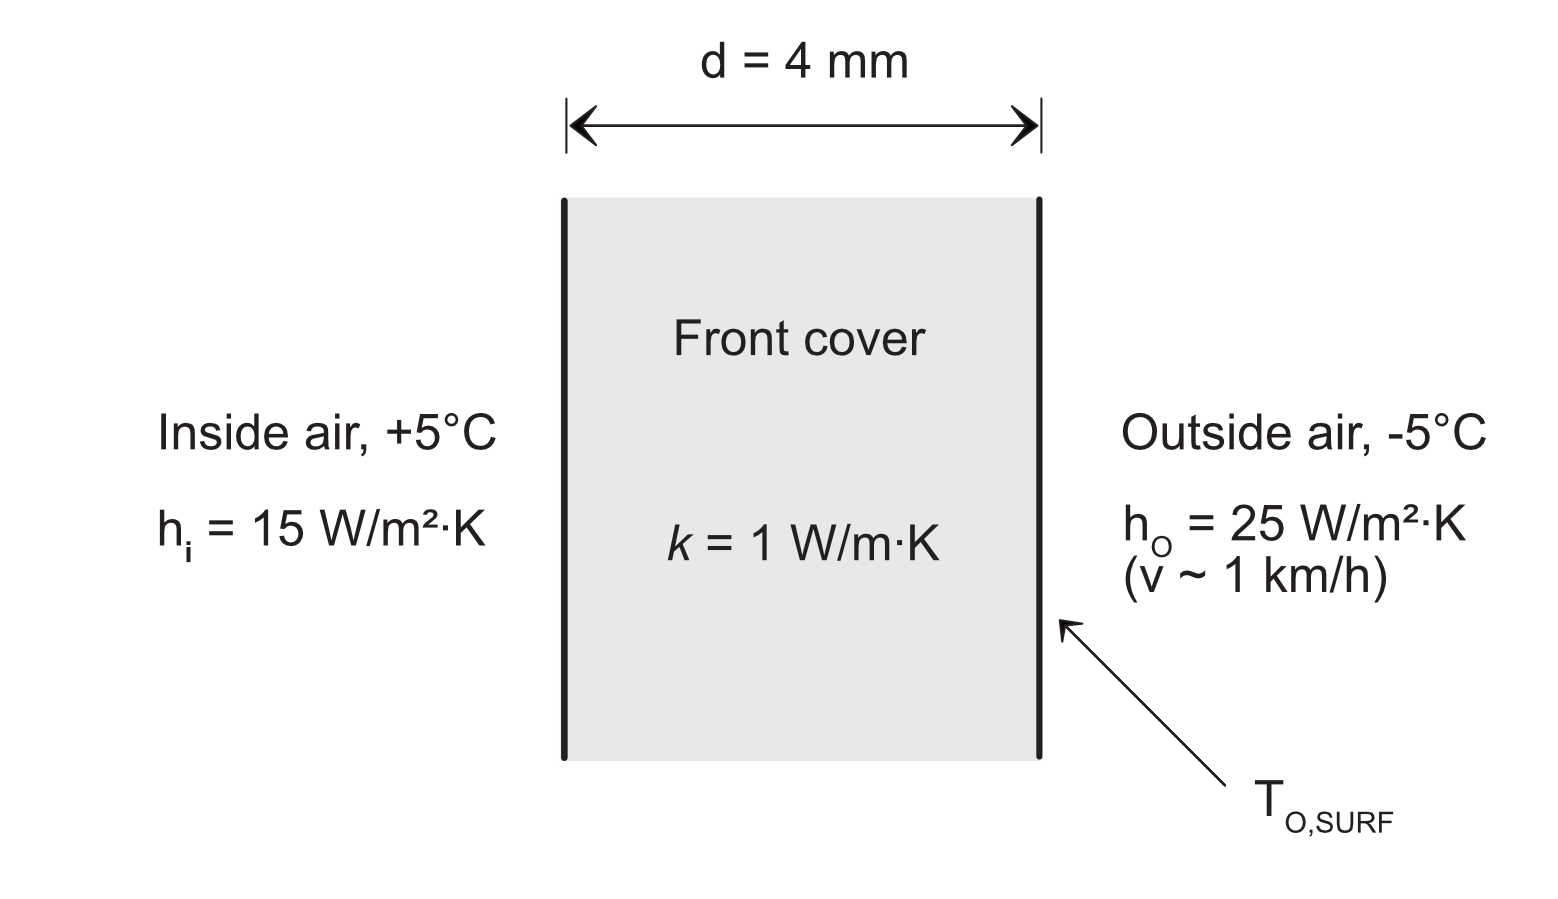
\includegraphics[scale=0.75]{\pathPics/Appendix_Windshield.png}
	\caption[PassiveHeating]{Side view sketch of a front cover}
	%\label{fig:fig1}
\end{figure}
The outer surface temperature is derived from the heat transfer rate per unit surface area, \(\dot{Q}/A\) and the thermal resistance of the front cover. The heat transfer rate per unit surface area corresponds to the power dissipated through the front cover area and can be estimated by weighting the power consumption of the sensor with the fraction of the surface area of the front cover to the surface area of the sensor. A sensor with a size of roughly 11 cm x 10 cm x 8.5 cm has a surface area of 580 \unit{cm²}. Assuming a front cover area of 45 \unit{cm^2} and an uniform dissipation loss through the sensor surface, then the sensor looses about 8 \unit{\%} of its power through the front cover:
\begin{equation}
P = 8 \% \cdot 5 \unit{W} = 0.4 \unit{W}
\end{equation}
This corresponds to a heat transfer rate per unit surface of 90 \unit{W/m²}. The temperature on the outer surface is then given by considering the heat transfer from the outer surface to the ambient air
\begin{equation}
T_{o,surf} = T_{o} + R_{o,conv}\cdot \frac{\dot{Q}}{A} = +5 \dC - 3.4 \dC = -1.4 \dC
\end{equation}
with the convection resistance \(R_{o,conv} = 1/h_{o,conv} = 0.04 \,\, \unit{m\cdot K/W}\). The temperature of the air inside the sensor can be derived in a similar manner,  
\begin{equation}
T_{i} = T_{o} + R_{tot}\cdot \frac{\dot{Q}}{A} = -5 \dC + 10 \dC = +5 \dC
\end{equation}
by considering the heat transfer through the front cover with a total resistance \(R_{tot} = 1/h_{i,conv}+d/k+1/h_{o,conv} = 0.11 \unit{m\cdot K/W}\).


\subsection{Heating Plate}


\subsection{3-D Thermal Simulation}
